
\documentclass[12pt,a4paper]{report}
\usepackage{graphicx}
\usepackage[utf8]{inputenc}
%%%%%%%%%%%%%%%%%%%%%%%%%%%%%%%%%%%%%%%%%%%%%%%%%%%%%%%%%%%%%%%%
% LaTeX code  to enable                                        %
% the build by XeLaTeX, specific for Malayalam language        %
%%%%%%%%%%%%%%%%%%%%%%%%%%%%%%%%%%%%%%%%%%%%%%%%%%%%%%%%%%%%%%%%
\usepackage{pdfpages}
\usepackage{fontspec}
\usepackage{polyglossia,xltxtra}
\setdefaultlanguage{malayalam}
\setmainfont[Script=Malayalam, HyphenChar="00AD]{Rachana}
\newfontfamily\engfont[Mapping=tex-text]{FreeSerif}
\newfontfamily\malayalamfontsf{Rachana}[Script=Malayalam]
\newfontfamily\malayalamfonttt{Rachana}[Script=Malayalam]
\def\xromn#1{{\fontencoding{T1}\fontfamily{cmr}\selectfont#1}}
\def\squote{\xromn{`}}
\def\esquote{\xromn{'}}
\def\dquote{\xromn{``}}
\def\edquote{\xromn{''}}
\DeclareTextFontCommand{\myfont}{\engfont}
\def\mdash{\myfont{\textemdash}}
\def\ndash{\myfont{\textendash}}
\lefthyphenmin=3
\righthyphenmin=4
\linespread{1.2}
\widowpenalty=10000
\clubpenalty=10000
\raggedbottom
\sloppy
%%%%%%%%%%%%%%%%%%%%%%%%%%%%%%%%%%%%%%%%%%%%%%%%%%%%%%%%%%%%%%%%
%                end of inserted code                          %
%%%%%%%%%%%%%%%%%%%%%%%%%%%%%%%%%%%%%%%%%%%%%%%%%%%%%%%%%%%%%%%%

\begin{document}
\begin{titlepage}
\thispagestyle{empty}

\vspace{0.2in}

\begin{center}
{\Huge{}expEYES-17}
\par\end{center}{\Huge \par}

\begin{center}
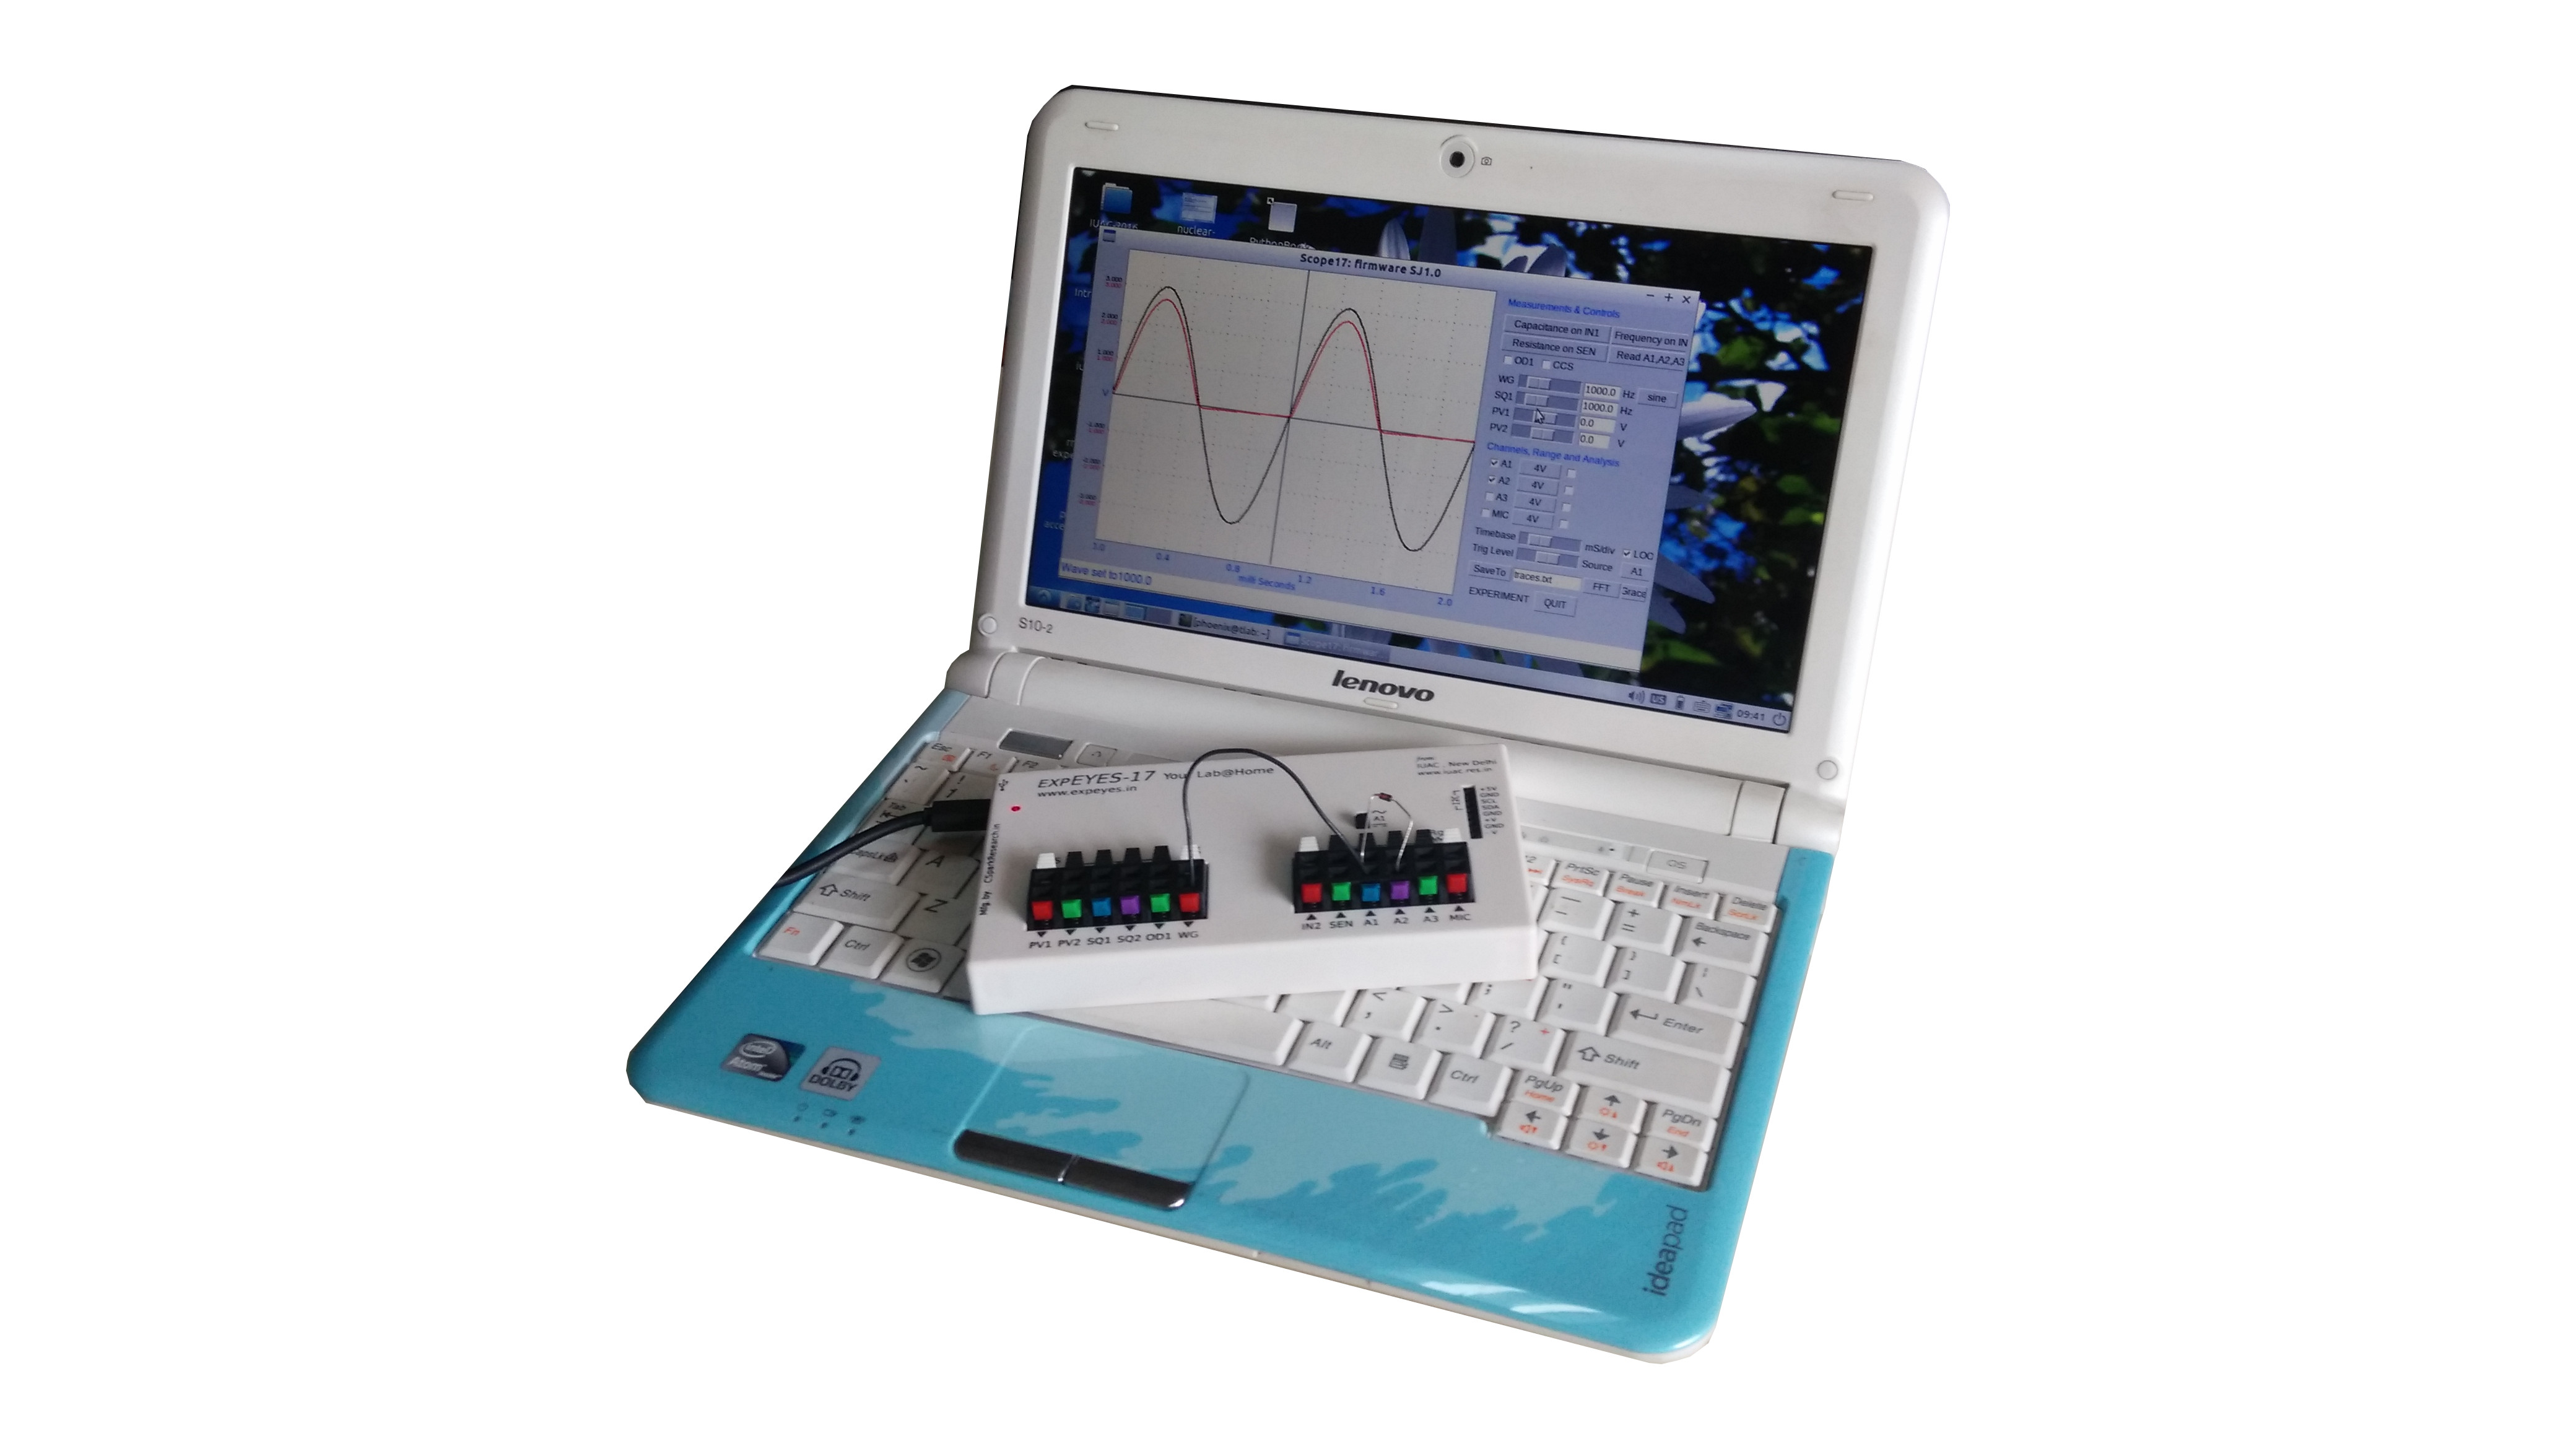
\includegraphics[width=6cm]{../../pics/eyes17-nb}
\par\end{center}

\begin{center}
{\large{}സഹായഗ്രന്ഥം  }
\par\end{center}{\large \par}

\begin{center}
{\LARGE{} യുവശാസ്ത്രജ്ഞർക്കും സാങ്കേതികവിദഗ്ദ്ധർക്കുമുള്ള}\\
{\LARGE{}  പരീക്ഷണങ്ങൾ }
\par\end{center}{\LARGE \par}

\begin{center}
http://expeyes.in
\par\end{center}

\begin{center}
from
\par\end{center}

\begin{center}
PHOENIXപ്രൊജക്റ്റ് \\
ഇന്റർ യൂണിവേഴ്സിറ്റി ആക്സിലറേറ്റർ സെന്റർ  \\
(UGCയുടെ ഒരു ഗവേഷണസ്ഥാപനം )\\
ന്യൂ ഡൽഹി  110 067\\
www.iuac.res.in
\par\end{center}

\end{titlepage}
\end{document}

